%卒業論文概要テンプレート ver. 1.0

\documentclass[uplatex,twocolumn,dvipdfmx]{jsarticle}
\usepackage[top=22mm,bottom=22mm,left=20mm,right=20mm]{geometry}
\setlength{\columnsep}{15mm}
\usepackage[T1]{fontenc}
\usepackage{txfonts}
\usepackage{wrapfig}
\usepackage[expert,deluxe]{otf}
\usepackage[dvipdfmx,hiresbb]{graphicx}
\usepackage[dvipdfmx]{hyperref}
\usepackage{pxjahyper}
\usepackage{secdot}

\makeatletter
\renewcommand{\section}{%
  \@startsection{section}{1}{\z@}%
  {0.6\Cvs}{0.4\Cvs}%
  {\normalfont\normalsize\raggedright}}
\renewcommand{\subsection}{\@startsection{subsection}{2}{\z@}%
  {\z@}{\z@}%
  {\normalfont\normalsize}}
\renewcommand{\subsubsection}{\@startsection{subsubsection}{3}{\z@}%
  {\z@}{\z@}%
  {\normalfont\normalsize}}
\makeatother
%ここから上を編集する必要はない.





%吉野君
\usepackage{here}

%タイトルと学生番号,名前だけ編集すること
\title{\vspace{-5mm}\fontsize{14pt}{0pt}\selectfont ビッグデータ処理技術を用いたWikipediaマイニング}
\author{\normalsize プロジェクトマネジメントコース・ソフトウェア開発管理グループ 矢吹研究室 1242005 石井康之}
\date{}
\pagestyle{empty}
\begin{document}
\fontsize{10.5pt}{\baselineskip}\selectfont
\maketitle





%以下が本文
\section{序論}


Wikipediaは,多くの人がボランティアで執筆するオンライン百科事典プロジェクトである.

Wikipediaは2001年1月15日に創設され,2001年5月ごろに日本語版が発足した.全てのオープンコンテキストの知識資源は無料で一般に提供されている.

多くの人が参加するプロジェクトの代表例であるWikipediaを調査することによって,このような形式のプロジェクトのマネジメントについての有意義な知見が得られることが期待できる.

このオープンなオンライン百科事典プロジェクトの成功理由について様々な考察がされており,その中の1つの要因に「適切な時に,それぞれのニッチに対しボトムアップとトップダウンの適切な混合率を出していた」というのがある\cite{bottom1}.
Wikipediaでは,ボトムアップの力,無統制の善良さで成長したと見えるのだが,実際にプロセスをよく調べてみると,その中心にはエリートがいて、見かけ以上に入念なトップダウンのしくみによる管理がなされている.

Wikipediaの編集者の中には,管理者と呼ばれる利用者たちがおり,この利用者たちがWikipediaの中心のエリートと呼ばれる人たちとして,統制を行っているのではないかと考えた.

そこで当研究では,管理者の動向を見るため,管理者の編集回数がどのように変化しているか調査する.結果からWikipediaの成功理由に,この管理者がどのように関係しているか見つけ出す.

\section{目的}

Wikipediaを一つのプロジェクトとみなし,このオンライン百科事典で管理者の動向がどのように変化しているか調査する.

\section{手法}

以下のとおり手法を行う.
\begin{enumerate}
 \item Wikipedia日本語版の編集履歴まで含んだファイルをダウンロードし,ローカルでデータマイニングを行う.
 \item Wikipediaの管理者の編集回数の変化を解析する.
 \item 管理者の編集の割合がプロジェクトの動きにどのようにつながっているのか調査する.
\end{enumerate}

\section{結果}

%図の挿入
\begin{figure}[H]
\centering
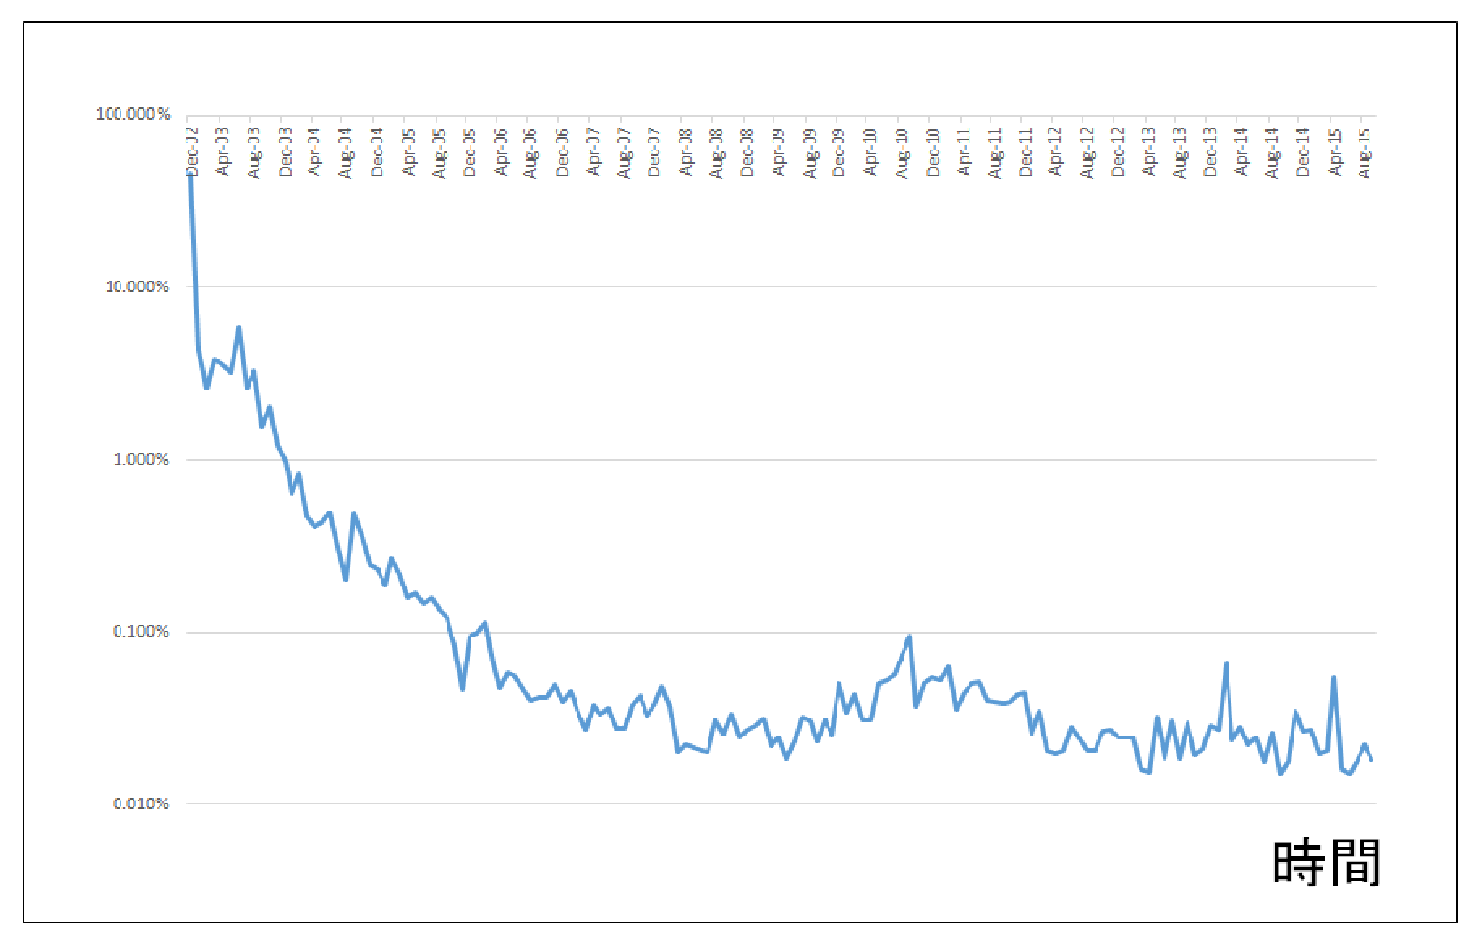
\includegraphics[width=7cm]{editors_per.png}
\caption{管理者の月別編集回数の割合の変化}\label{サンプル図}
\end{figure}


日本語版Wikipediaが実装されてからの,管理者の編集回数のデータ解析を行った.年々減少傾向になっている.


\section{考察}

日本語版Wikipediaでは,管理者が編集を行う必要性が薄れてきている.管理者の月別編集回数の割合によれば,Wikipedia実装当初の2002年2月ごろでは,全体の約5割ほど占めていたが,2007年8月ごろからは,安定して低い割合で運用しているからである.

\section{結論}

日本語版Wikipediaの,管理者の編集回数は元々行う割合が低く,また年々減少傾向にあった.

\bibliographystyle{junsrt}
\bibliography{biblio}%「biblio.bib」というファイルが必要.

\end{document}